\documentclass[11pt,a4paper]{article}
%%%%%%%%%%%%%%%%%%%%%%%%%%%%%%%%%%%%%%%%%%%%%%%%%%%%%%%%
%                      PACKAGES                        %
%%%%%%%%%%%%%%%%%%%%%%%%%%%%%%%%%%%%%%%%%%%%%%%%%%%%%%%%

\usepackage[utf8]{inputenc}
\usepackage{graphicx} % Allows you to insert figures
\usepackage[export]{adjustbox}
\usepackage{booktabs}
\usepackage{amsmath} % Allows you to do equations
\usepackage{helvet}
\usepackage{hyperref}
\renewcommand{\familydefault}{\sfdefault}
\usepackage[a4paper, total={6.5in, 9.5in}]{geometry} % Formats the paper size, orientation, and margins
\linespread{1.1} % about 1.5 spacing in Word
\setlength{\parindent}{0pt} % no paragraph indents
\setlength{\parskip}{1em} % paragraphs separated by one line
\usepackage{listings}
\usepackage{enumitem}
\usepackage{xcolor}
\usepackage{hyperref}
\hypersetup{
	colorlinks=true,
	urlcolor=cyan,
	linktoc=none,
}
\usepackage{fancyhdr}
\pagestyle{fancy}
\fancyhead[L,C,R]{}
\fancyfoot[L]{Occupi - Office Capacity Predictor}
\fancyfoot[C]{}
\fancyfoot[R]{\textbf{\thepage}}
\renewcommand{\headrulewidth}{0pt}
\renewcommand{\footrulewidth}{0.5pt}

\definecolor{codegreen}{rgb}{0,0.6,0}
\definecolor{codegray}{rgb}{0.5,0.5,0.5}
\definecolor{codepurple}{rgb}{0.58,0,0.82}
\definecolor{backcolour}{rgb}{0.95,0.95,0.92}

\lstdefinestyle{mystyle}{
backgroundcolor=\color{backcolour},
commentstyle=\color{codegreen},
keywordstyle=\color{magenta},
numberstyle=\tiny\color{codegray},
stringstyle=\color{codepurple},
basicstyle=\ttfamily\footnotesize,
breakatwhitespace=false,
breaklines=true,
keepspaces=true,
numbers=left,
numbersep=5pt,
showspaces=false,
showstringspaces=false,
showtabs=false,
tabsize=2,
}

\lstset{style=mystyle}
\def\code#1{\texttt{#1}}

%%%%%%%%%%%%%%%%%%%%%%%%%%%%%%%%%%%%%%%%%%%%%%%%%%%%%%%%
%            TITLE PAGE & TABLE OF CONTENTS            %
%%%%%%%%%%%%%%%%%%%%%%%%%%%%%%%%%%%%%%%%%%%%%%%%%%%%%%%%

\begin{document}
\begin{titlepage}
    \centering
    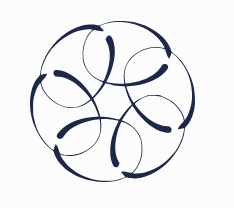
\includegraphics[width=0.4\textwidth]{logo-white.png}\par\vspace{1cm}
    {\scshape\LARGE Python Coding Standards\par}
    \vspace{1.5cm}
    {\huge\bfseries Occupi - Office Capacity Predictor\par}
    \vspace{2.5cm}
    \begin{tabular}{|c|c|}
        \hline
        \textbf{Name}      & \textbf{Student Number} \\
        \hline
        Rethakgetse Manaka & u22491032               \\
        Kamogelo Moeketse  & u22623478               \\
        Michael Chinyama   & u21546551               \\
        Tinashe Austin     & u21564176               \\
        Carey Mokou        & u21631532               \\
        \hline
    \end{tabular}
    \vfill
    {\large September 01, 2024\par}
\end{titlepage}

\tableofcontents
\pagebreak

%%%%%%%%%%%%%%%%%%%%%%%%%%%%%%%%%%%%%%%%%%%%%%%%%%%%%%%%
%                MAIN DOCUMENT CONTENT                 %
%%%%%%%%%%%%%%%%%%%%%%%%%%%%%%%%%%%%%%%%%%%%%%%%%%%%%%%%

\section*{Introduction}
\addcontentsline{toc}{section}{Introduction}
This document outlines the Python coding standards to ensure consistent, readable, and maintainable code. Following these standards will help all contributors write clean, efficient, and bug-free Python code.

\section*{General Code Structure}
\addcontentsline{toc}{section}{General Code Structure}
All code should be clean, readable, and maintainable. Key practices include:
\begin{itemize}
    \item Using meaningful names for variables, functions, and classes.
    \item Follow consistent indentation with 4 spaces per level.
    \item Organize imports at the top of each file, grouping standard library imports, third-party imports, and local imports separately.
\end{itemize}

\section*{PEP 8 Compliance}
\addcontentsline{toc}{section}{PEP 8 Compliance}
All Python code must follow the PEP 8 style guide:
\begin{itemize}
    \item Line length should not exceed 79 characters.
    \item Use spaces around operators (e.g., `x = 5`, not `x=5`).
    \item Include a blank line between function definitions and after class declarations.
    \item Avoid unnecessary blank lines inside functions.
\end{itemize}

\section*{Error Handling and Logging}
\addcontentsline{toc}{section}{Error Handling and Logging}
Ensure code is resilient and provides meaningful error messages:
\begin{itemize}
    \item Use try-except blocks for any potentially unsafe operations.
    \item Always log errors using the `logging` module rather than `print`.
    \item Catch specific exceptions, not generic ones (e.g., `except ValueError` instead of `except`).
\end{itemize}

\section*{Functions and Methods}
\addcontentsline{toc}{section}{Functions and Methods}
Functions should be small, focused, and easy to understand:
\begin{itemize}
    \item Use descriptive names for functions and methods.
    \item Include type hints for function arguments and return values where appropriate.
    \item Each function should accomplish one specific task.
    \item Comment functions and methods with a brief description of what they do.
\end{itemize}

\section*{Code Comments and Documentation}
\addcontentsline{toc}{section}{Code Comments and Documentation}
All public functions, classes, and methods must have docstrings:
\begin{itemize}
    \item Use multi-line docstrings for functions and classes.
    \item Use inline comments sparingly and only when the code is non-obvious.
    \item Document any external libraries or APIs used.
    \item Write descriptive comments that explain the why, not the how.
\end{itemize}

\section*{Code Example}
\addcontentsline{toc}{section}{Code Example}
Example of a well-documented Python function:
\begin{lstlisting}
def get_predictions(data: Dict[str, Any]) -> List[float]:
    """
    Fetch predictions from the model.

    Args:
        data (dict): Input data for the model.

    Returns:
        list: Model predictions as a list of floats.
    """
    return model.predict(data)
\end{lstlisting}
\pagebreak

\section*{Testing and Debugging}
\addcontentsline{toc}{section}{Testing and Debugging}
Ensure that all critical functions are tested and debugged properly:
\begin{itemize}
    \item Write unit tests using `unittest` or `pytest` for each function.
    \item Use mock data where necessary, especially when handling external services.
    \item Use assertions in tests to validate function outputs.
\end{itemize}

\section*{References}
\addcontentsline{toc}{section}{References}
For more details on Python coding standards, please refer to:
\begin{itemize}
    \item PEP 8: \href{https://www.python.org/dev/peps/pep-0008/}{Python Enhancement Proposal 8 - Style Guide for Python Code}
    \item Python Documentation: \href{https://docs.python.org/3/}{Official Python Documentation}
\end{itemize}

\end{document}
